\documentclass[border=4pt]{standalone}
\usepackage{amsmath,amssymb,tikz}
\usetikzlibrary{arrows.meta}
\definecolor{figB}{RGB}{31,90,166}\definecolor{figR}{RGB}{176,48,48}
\begin{document}
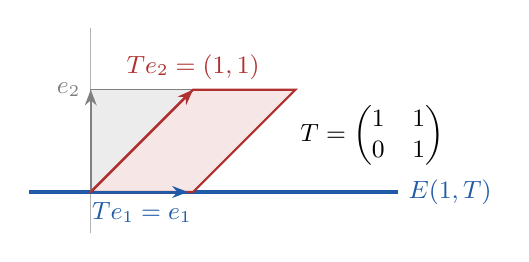
\begin{tikzpicture}[scale=1.3,>={Stealth[length=2mm]}]
\draw[gray!60] (-0.6,0)--(3.0,0); \draw[gray!60] (0,-0.4)--(0,1.6);
\draw[very thick,figB] (-0.6,0)--(3.0,0) node[right,font=\small]{$E(1,T)$};
\fill[gray!15] (0,0) rectangle (1,1); \draw[gray] (0,0) rectangle (1,1);
\fill[figR!12] (0,0)--(1,0)--(2,1)--(1,1)--cycle; \draw[figR,thick] (0,0)--(1,0)--(2,1)--(1,1)--cycle;
\draw[->,thick,figB] (0,0)--(0.95,0) ; 
\draw[->,thick,gray] (0,0)--(0,1) node[left,font=\small]{$e_2$};
\draw[->,thick,figR] (0,0)--(1,1) node[above,font=\small]{$Te_2=(1,1)$};
\node[figB,font=\small] at (0.5,-0.2) {$Te_1=e_1$};
\node[font=\small] at (2.75,0.55) {$T=\begin{pmatrix}1&1\\0&1\end{pmatrix}$};
\end{tikzpicture}
\end{document}
